\subsection{Hypotheses and Limitations}
\label{sec:thesis_hypotheses}
This section presents the hypotheses made on the context in order to limit the
scope of this thesis, as well as the reason behind these limitations and, when
applicable, how these could be removed in future works.

The first scope restrictions stem from the aeronautical context. Indeed:
\begin{itemize}
\item Only COTS architectures are considered. The use of self-made hardware is
not deemed acceptable in critical systems such as avionics.
\item Uses cache coherence. Using multi-core processors without cache coherence
prevents any gain they would otherwise provide over single-core processors when
running application with parallel processing.
\item Snooping-based cache coherence. This is the more common approach to cache
coherence in COTS, and thus makes for a good starting point. Extending this
thesis to also handle directory-based cache coherence would require the creation
of a different architecture model.
\end{itemize}

Other restrictions are more related to what the thesis' time constraints
permitted. The focus stayed on cache coherence itself, since this is what the
existing literature consistently avoids. Thus, elements that are already
explored in other numerous works have not been expended upon past the bare
minimum. An example of architecture complying with these restrictions can
be seen in Figure~\ref{fig:second_intro:typical_arch}.

\begin{figure}[hbt!]
\begin{center}
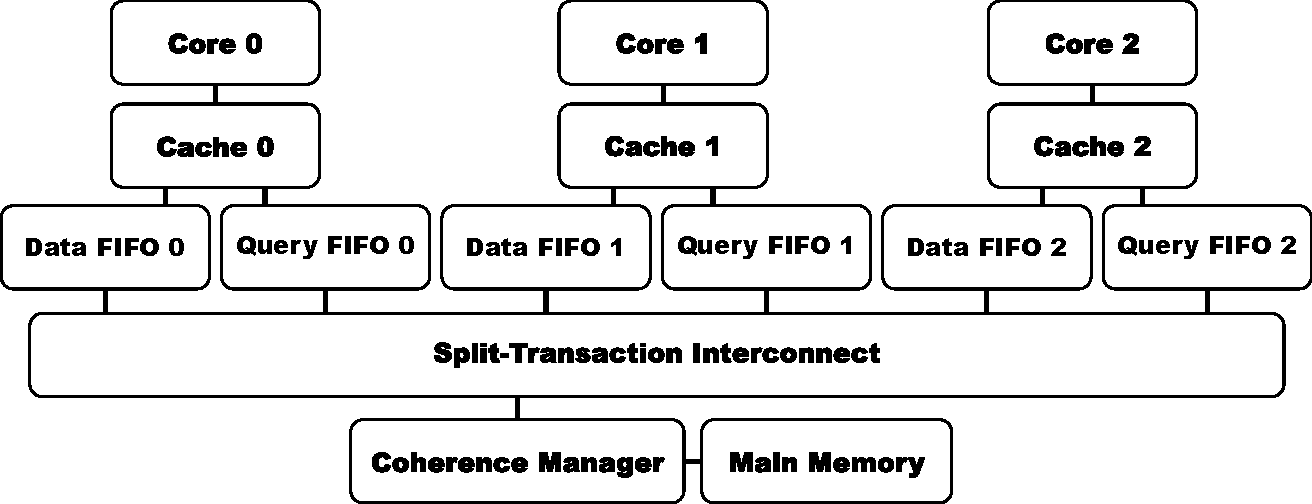
\includegraphics[width=\textwidth]{\chapterdirectory/figure/typical_arch3.pdf}
\end{center}
\caption{Typical profile of the targeted architecture}
\label{fig:second_intro:typical_arch}
\end{figure}

\begin{itemize}
\item No cache hierarchy. The coherence is studied within a single level of
cache, there is no issue of memory element propagation across L1, L2, or L3
caches. Adding proper support for cache hierarchy to the tools presented in this
thesis would require a large number of modifications.
\item One core per cache. The solution proposed in this thesis does not properly
handle multiple cores per cache, as the model fails to account for the
originator of each request in at least one of its functionalities. Unless as of
yet unknown issues arise, this limitation should be fairly easily removed.
\item Fully associative cache placement policy. Supporting the segregation of
cache lines would add a layer of complexity without being a fundamental change
in what the tools prove to be possible. Allowing configuration by the user so
that other placement policies may be used should be straight forward, and is
only absent because of its low priority.
\item LRU cache replacement policy. While a replacement policy had to be chosen,
the most popular one, PLRU, was not the one implemented. LRU is easier to
debug, which is why it was chosen. Here also, adding support for other policies
would not constitute a major change in the model, but neither was it considered
a high priority feature.
\item Simplified program representation. The focus is really put on cache
coherence. No matter how complex, programs only interact with cache coherence
through memory accesses. Thus, only sequences of memory accesses are represented
and, by default, instruction jumping and branching is not supported.
Technically, this can already be bypassed by creating a new automaton for each
of the more complex program, however, automation of the automaton creation is
required before such a solution can be considered reasonable.
\end{itemize}

Lastly, the tools proposed in this thesis only constitute part of the solution
needed to properly analyse multi-core processors for use in avionics:
\begin{itemize}
\item Results focused on cache coherence only. For accurate measurement of the
effects of interference on applications running in a multi-core, the separate
analysis of sources of interference is inadequate as not only are these sources
not independent, but the effects of each source interference can, by definition,
alter the behavior of the application and thus lead to the other sources of
interference having a different effect on the application. Assuming a worst case
for each source of interference does not ensure that the global worst case is
measured (a principle known as \textit{timing anomaly}). Thus, the contributions
made in this thesis would need to be integrated into an all-encompassing
framework in order to allow adequate estimation of the WCET.
\end{itemize}

\subsection{Framework Overview}
\label{sec:second_intro:framework}
Figure~\ref{fig:second_intro:approach} presents the general framework proposed
in this thesis for the analysis of the impact of cache coherence on software
running on a multi-core COTS system.

Given an architecture, the applicant performs an identification of the cache
coherence mechanisms. This removes any ambiguities that may be lingering in the
description of the cache coherence protocol from the architecture's
documentation. This process is described in
Chapter~\ref{cha:identifying_cache_coherence} and involves the use of
performance monitors in order to observe the behavior of the architecture's
cache coherence mechanisms and compare it with that of a hypothetical cache
coherence protocol. If the two match, the applicant thus obtains an
ambiguity-free cache coherence protocol description for the architecture.

Using this ambiguity-free cache coherence protocol, the temporal cost of each
operation is quantified through benchmarks. Indeed, now that all relevant
coherence states and behaviors are known, the applicant can be sure their
measures are not missing important results. This step is not expanded upon by
the thesis, as the existing literature already covers it (see
Chapter~\ref{cha:micro-benchs}). With these measures, a profile of the
architecture's cache coherence mechanisms has been obtained.

To evaluate the impact of cache coherence on the execution of software, this
thesis proposes the use of formal methods. This requires the creation of a model
for the architecture (see Chapter~\ref{cha:modeling_cache_coherence}), as well
as the definition of the appropriate queries in order to retrieve information
that can be used by the applicant through model checking (see
Chapter~\ref{chap:exposing_interference}).

\begin{figure}[hbt!]
\iffalse
\begin{subfigure}[t]{\textwidth}
\centering
\begin{tikzpicture}[
  font=\sffamily,
  every matrix/.style={ampersand replacement=\&,column sep=2.5cm,row sep=1cm},
  source/.style={draw,thick,rounded corners,fill=yellow!20,inner sep=.3cm},
  process/.style={draw,thick,circle,fill=blue!20},
  sink/.style={source,fill=green!20},
  datastore/.style={draw,very thick,shape=datastore,inner sep=.3cm},
  dots/.style={gray,scale=2},
  to/.style={->,>=stealth',shorten >=1pt,semithick,font=\sffamily\footnotesize},
  every node/.style={align=center}]

  % Position the nodes using a matrix layout
  \matrix{
    \node[datastore] (architecture) {Architecture};
      \& \node[sink] (identification) {%
         \begin{tabular}{@{}c@{}}
            Cache Coherence Identification\\
            (Chapter~\ref{cha:identifying_cache_coherence})
         \end{tabular}
         };
      \&
    \node[datastore] (cacheprotocol) {%
         \begin{tabular}{@{}c@{}}
            Cache Coherence\\ Protocol
         \end{tabular}
         };
      \\
  };

  % Draw the arrows between the nodes and label them.
  \draw[to] (architecture) to (identification);

  \draw[to] (identification) to (cacheprotocol);
\end{tikzpicture}

\end{subfigure}
\begin{subfigure}[t]{\textwidth}
\vspace{2em}
\centering
\begin{tikzpicture}[
  font=\sffamily,
  every matrix/.style={ampersand replacement=\&,column sep=2.5cm,row sep=1cm},
  source/.style={draw,thick,rounded corners,fill=yellow!20,inner sep=.3cm},
  process/.style={draw,thick,circle,fill=blue!20},
  sink/.style={source,fill=green!20},
  datastore/.style={draw,very thick,shape=datastore,inner sep=.3cm},
  dots/.style={gray,scale=2},
  to/.style={->,>=stealth',shorten >=1pt,semithick,font=\sffamily\footnotesize},
  every node/.style={align=center}]

  % Position the nodes using a matrix layout
  \matrix{
   \&
    \node[datastore] (cacheprotocol) {%
         \begin{tabular}{@{}c@{}}
            Cache Coherence\\ Protocol
         \end{tabular}
         };
      \&
   \\
    \node[datastore] (architecture) {Architecture};
      \&
      \node[source] (benchmarking) {%
         \begin{tabular}{@{}c@{}}
            Benchmarking\\
            (Chapter~\ref{cha:micro-benchs})
         \end{tabular}
      };
      \&
    \node[datastore] (cacheperformance) {%
         \begin{tabular}{@{}c@{}}
            Cache Coherence\\
            Performance
         \end{tabular}
      };
      \\
  };

  % Draw the arrows between the nodes and label them.
  \draw[to] (architecture) to (benchmarking);
  \draw[to] (cacheprotocol) to (benchmarking);

  \draw[to] (benchmarking) to (cacheperformance);
\end{tikzpicture}

\end{subfigure}
\begin{subfigure}[t]{\textwidth}
\vspace{4em}
\centering
\begin{tikzpicture}[
  font=\sffamily,
  every matrix/.style={ampersand replacement=\&,column sep=2.5cm,row sep=1cm},
  source/.style={draw,thick,rounded corners,fill=yellow!20,inner sep=.3cm},
  process/.style={draw,thick,circle,fill=blue!20},
  sink/.style={source,fill=green!20},
  datastore/.style={draw,very thick,shape=datastore,inner sep=.3cm},
  dots/.style={gray,scale=2},
  to/.style={->,>=stealth',shorten >=1pt,semithick,font=\sffamily\footnotesize},
  every node/.style={align=center}]

  % Position the nodes using a matrix layout
  \matrix{
   \node[datastore] (application) {Application};
   \&
    \node[datastore] (cacheprotocol) {%
         \begin{tabular}{@{}c@{}}
            Cache Coherence\\ Protocol
         \end{tabular}
         };
      \&
   \\
      \&
      \node[sink] (uppaal) {
         \begin{tabular}{@{}c@{}}
            UPPAAL Analysis\\
            (Chapters~\ref{cha:modeling_cache_coherence} and
            \ref{chap:exposing_interference})
         \end{tabular}
         };
      \&
      \node[datastore] (coherenceeffect) {%
         \begin{tabular}{@{}c@{}}
            Cache Coherence\\
            Impact
         \end{tabular}
      };
      \\
    \node[datastore] (architecture) {Architecture};
    \& \node[datastore] (cacheperformance) {%
         \begin{tabular}{@{}c@{}}
            Cache Coherence\\
            Performance
         \end{tabular}
      };
   \\
  };

  % Draw the arrows between the nodes and label them.

  \draw[to] (architecture) to (uppaal);
  \draw[to] (cacheperformance) to (uppaal);
  \draw[to] (cacheprotocol) to (uppaal);
  \draw[to] (application) to (uppaal);

  \draw[to] (uppaal) to (coherenceeffect);
\end{tikzpicture}

\end{subfigure}
\fi
\centering
\begin{tikzpicture}[
  font=\sffamily,
  every matrix/.style={ampersand replacement=\&,column sep=2.5cm,row sep=1cm},
  source/.style={draw,thick,rounded corners,fill=yellow!20,inner sep=.3cm},
  process/.style={draw,thick,circle,fill=blue!20},
  sink/.style={source,fill=green!20},
  datastore/.style={draw,very thick,shape=datastore,inner sep=.3cm},
  dots/.style={gray,scale=2},
  to/.style={->,>=stealth',shorten >=1pt,semithick,font=\sffamily\footnotesize},
  every node/.style={align=center}]

  % Position the nodes using a matrix layout
  \matrix{
    \node[datastore] (architecture) {Architecture};
      \& \node[sink] (identification) {%
         \begin{tabular}{@{}c@{}}
            Cache Coherence Identification\\
            (Chapter~\ref{cha:identifying_cache_coherence})
         \end{tabular}
         };
      \&
    \node[datastore] (cacheprotocol) {%
         \begin{tabular}{@{}c@{}}
            Cache Coherence\\ Protocol
         \end{tabular}
         };
      \\


   \&
      \&
   \\
      \&
      \node[source] (benchmarking) {%
         \begin{tabular}{@{}c@{}}
            Benchmarking\\
            (Chapter~\ref{cha:micro-benchs})
         \end{tabular}
      };
      \&
    \node[datastore] (cacheperformance) {%
         \begin{tabular}{@{}c@{}}
            Cache Coherence\\
            Performance
         \end{tabular}
      };
      \\



   \&
      \&
   \\
      \node[datastore] (application) {Application};
      \&
      \node[sink] (uppaal) {
         \begin{tabular}{@{}c@{}}
            UPPAAL Analysis\\
            (Chapters~\ref{cha:modeling_cache_coherence} and
            \ref{chap:exposing_interference})
         \end{tabular}
         };
      \&
      \node[datastore] (coherenceeffect) {%
         \begin{tabular}{@{}c@{}}
            Cache Coherence\\
            Impact
         \end{tabular}
      };
   \\
  };

  % Draw the arrows between the nodes and label them.
  \draw[to] (architecture) to (identification);

  \draw[to] (identification) to (cacheprotocol);



  \draw[to] (architecture) to (benchmarking.north west);
  \draw[to] (cacheprotocol) to (benchmarking.north east);

  \draw[to] (benchmarking) to (cacheperformance);



  \draw[to] (architecture) to (uppaal.north west);
  \draw[to] (cacheperformance) to (uppaal.north east);
  \draw[to] (cacheprotocol) to (uppaal);
  \draw[to] (application) to (uppaal);

  \draw[to] (uppaal) to (coherenceeffect);
\end{tikzpicture}

\caption{Approach Overview}
\label{fig:second_intro:approach}
\end{figure}
